\documentclass[11pt]{article}  
\usepackage[margin=1in]{geometry}
\parindent=0in
\parskip=8pt
\usepackage{fancyhdr,amssymb,amsmath, graphicx, listings,float,subfig,enumerate,epstopdf,color,multirow,setspace,bm,textcomp}
\usepackage[usenames,dvipsnames]{xcolor}
\usepackage{hyperref}
\usepackage{graphicx}
\graphicspath{{./Images}}

\pagestyle{fancy}


\begin{document} 

\lhead{Assignment \# 3}
\chead{Robert Denim Horton}
\rhead{\today}

\begin{center}\begin{Large}
CS 4720/5720 Design and Analysis of Algorithms

Homework \#3

Student: (Robert Denim Horton)
\end{Large}
\end{center}


\section*{Answers to homework problems:}

\begin{enumerate}
\setcounter{enumi}{1}
% Question 2
\item Consider the network shown in Figure 5.18: there is an edge between each pair of nodes, with five of the edges corresponding to positive relationships, and the other five of the edges corresponding to negative relationships.\\\\
% Uncomment to insert picture from Homeworkxx/Images
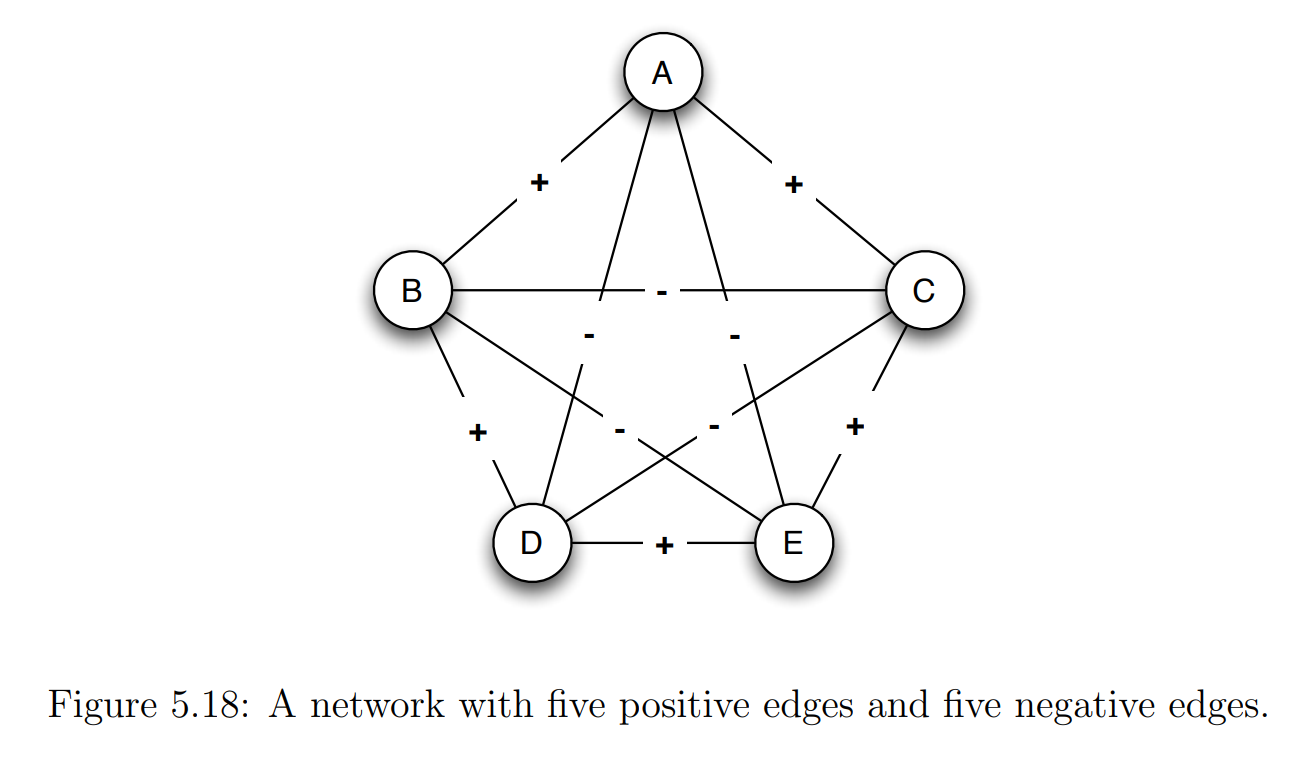
\includegraphics[scale=1]{Figure_5_18}\\
Each edge in this network participates in three triangles: one formed by each of the additional nodes who is not already an endpoint of the edge. (For example, the A-B edge participates in a triangle on A, B, and C, a triangle on A, B, and D, and a triangle on A, B, and E. We can list triangles for the other edges in a similar way.)\\\\
For each edge, how many of the triangles it participates in are balanced, and how many are unbalanced. (Notice that because of the symmetry of the network, the answer will be the same for each positive edge, and also for each negative edge; so it is enough to consider this for one of the positive edges and one of the negative edges.\\\\
\textcolor{gray}{
Answer:\\
From the formal definition given in class and in chapter 5, a connection between two nodes can be considered either a positive edge of a negative edge.  For the sake of this class we consider a complete graph to have the \textit{Structural Balance Property} if for every set of 3 nodes in the graph, the 3 nodes are connected with edges that are either all positive or exactly one edge is positive and the other two are negative. In Figure 3.1 we see several examples of graphs labelled either balanced or unbalanced.  Each graph is labelled as such representing balanced graph as graphs that have an structure balance property.\\
\begin{center}
	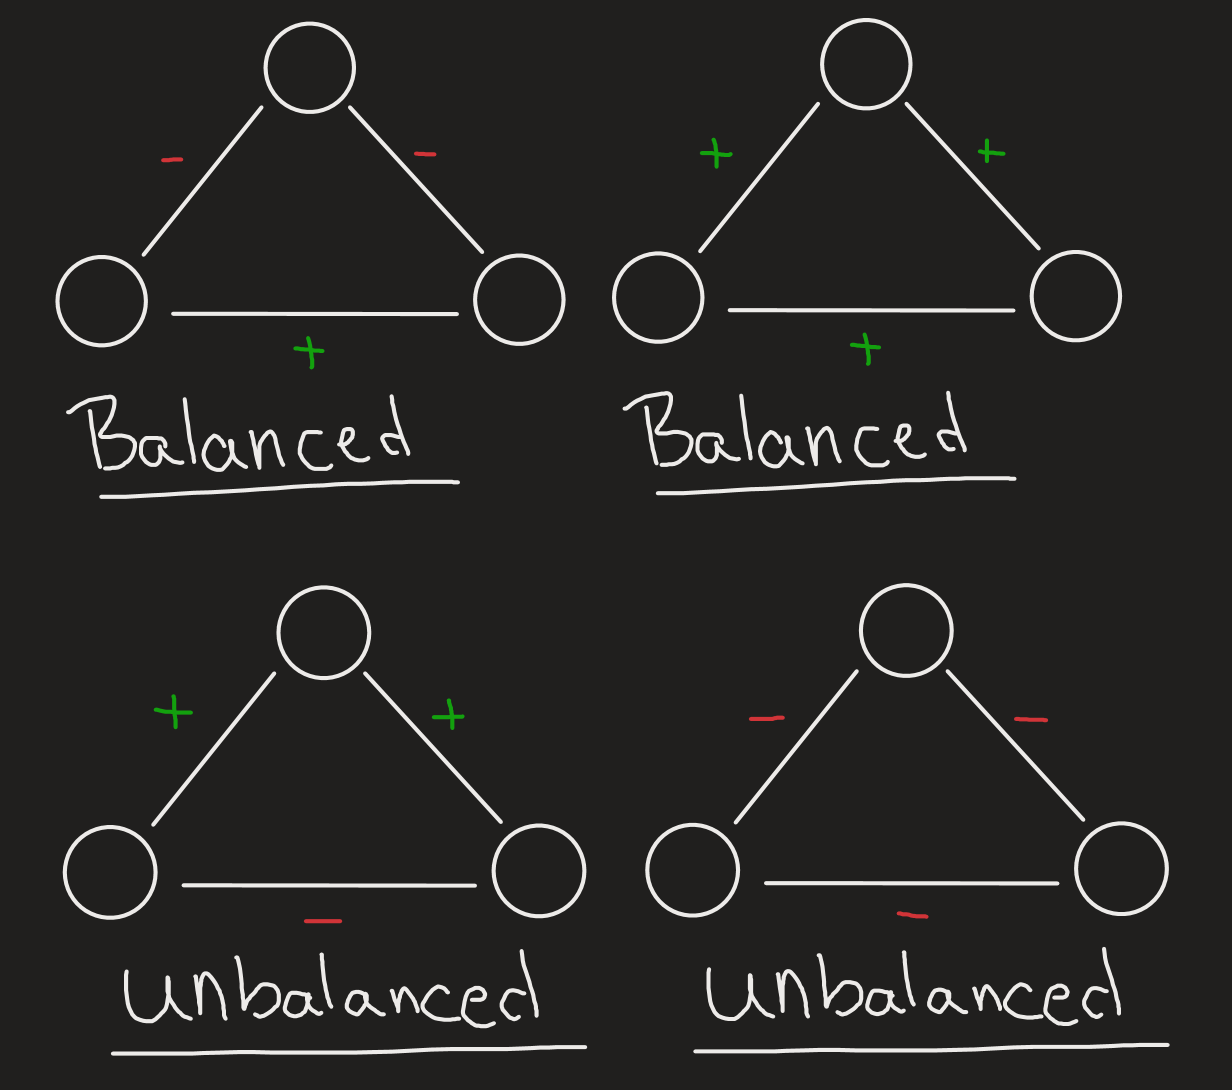
\includegraphics[scale=0.5]{example_ballanced_and_not_ballanced_graph}\\
\end{center}
Now with the established definition and visual examples it is easier to show how many balanced and unbalanced triangles exists for each edge in Figure 5.18. Due to the symmetry From Figure 3.2 we can simply look at one positive edge and one negative edge and assume the same for every positive and negative edge. Looking at the positive edge between nodes D and E we now evaluate each possibly triangle with this edge as its base.  So nodes D, E, and B  form the graph shown in the following Figure 3.2.1.\\
\begin{center}
	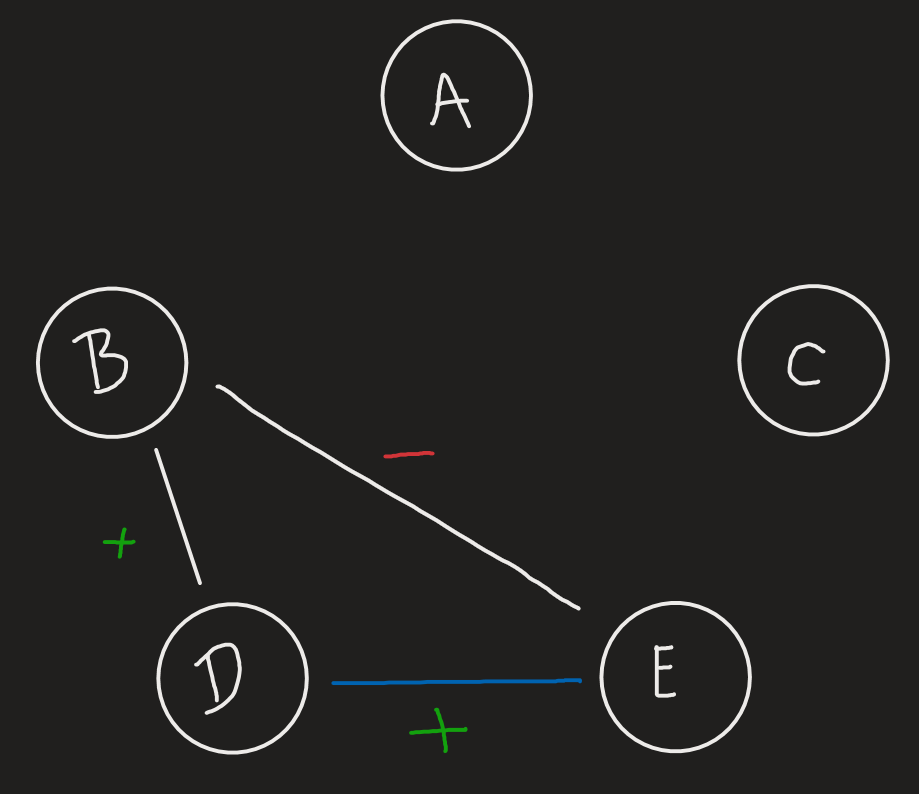
\includegraphics[scale=0.5]{Figure_3_2_1}\\
\end{center}
here we see that there is two positive connections, between nodes D and E and nodes D and B.  There is one negative edge between nodes E and B. For triangle formed by nodes D, E, and A we get the graph in Figure 3.2.2.
\begin{center}
	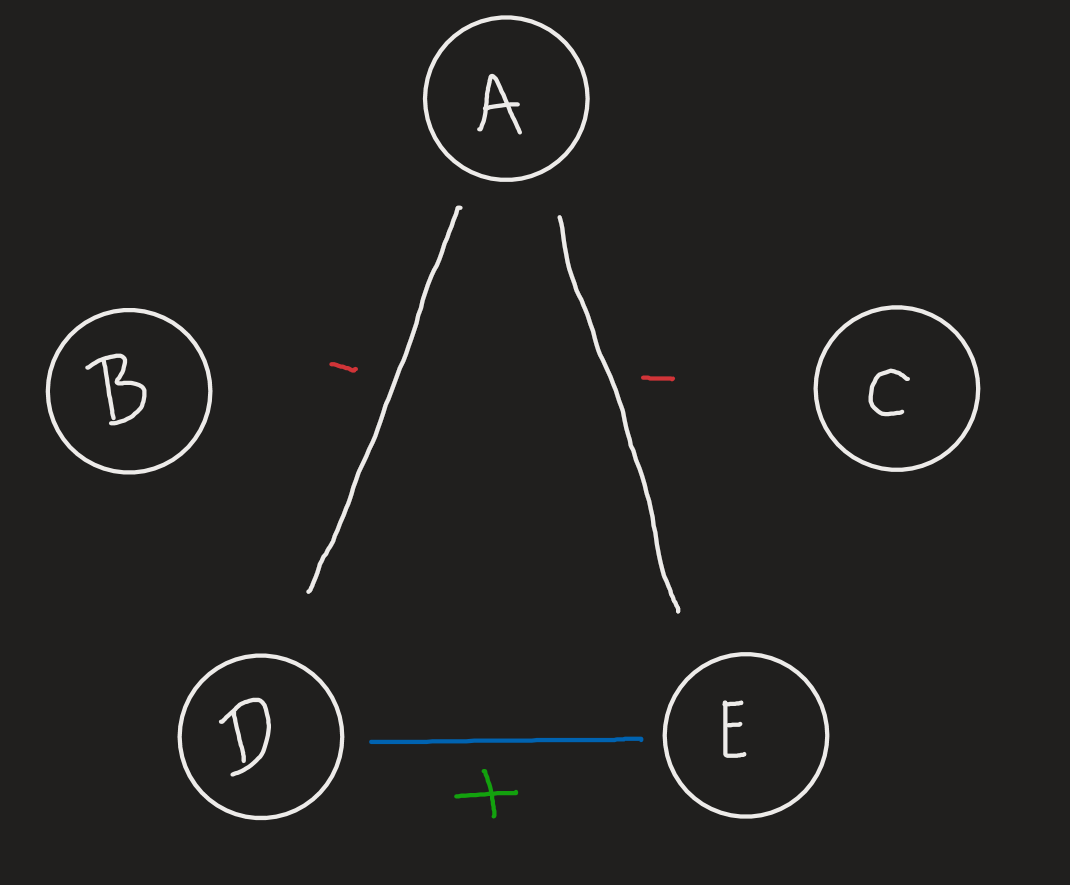
\includegraphics[scale=0.5]{Figure_3_2_2}\\
\end{center}
Here we see one positive connections and two negative edges. The negative edges include the edge between nodes A and D and between nodes A and E.  The only positive edge is between the nodes D and E. For the last triangle, that shares and edge with D and E we have a shared connection to node C.  So for the triangle formed by nodes D, E, and C we get the graph in Figure 3.2.3.
\begin{center}
	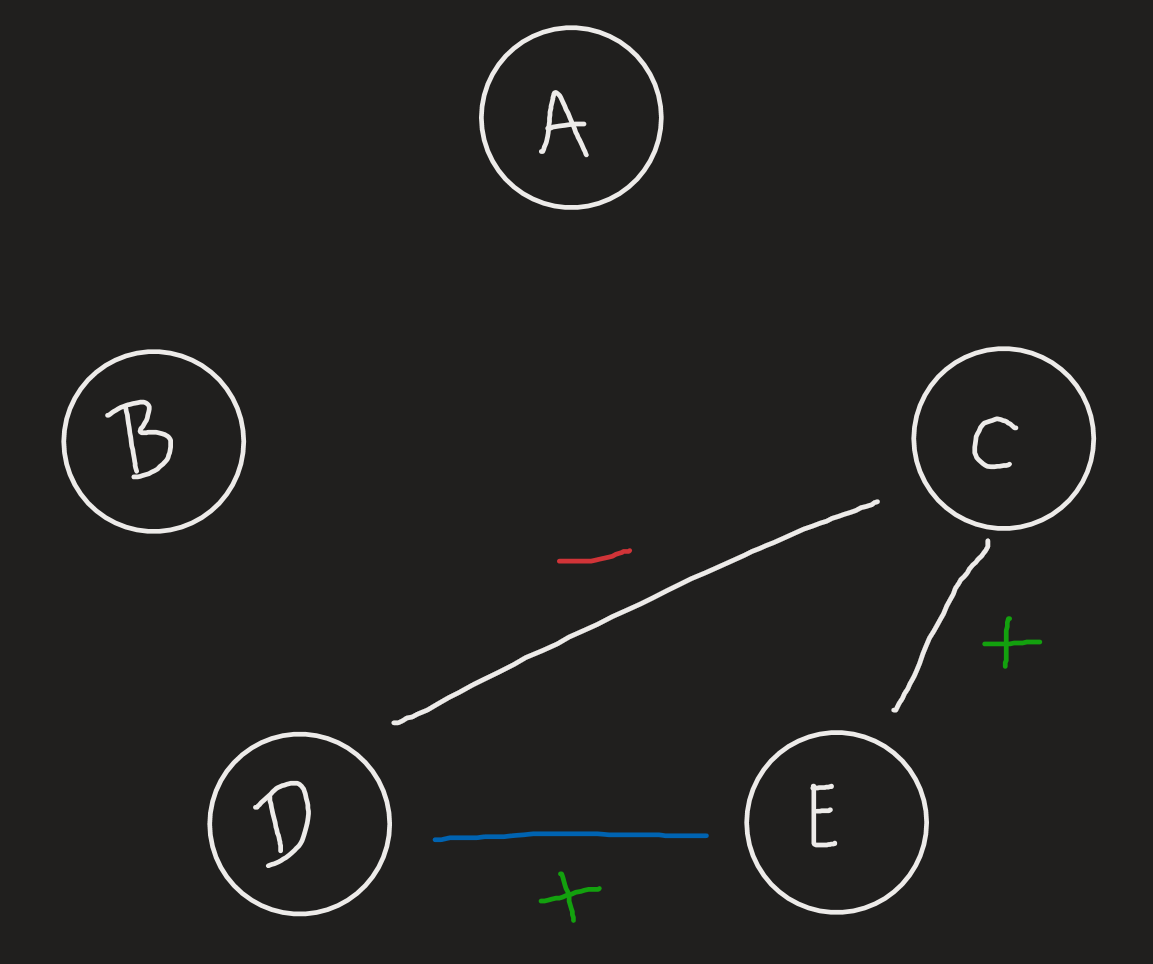
\includegraphics[scale=0.5]{Figure_3_2_3}\\
\end{center}
Once again we see two positive connections and one negative edge. The negative edge is along the inside edge between nodes D and C.  The positive edges include the base edge between nodes D and E, and the second positive edge is between nodes E and C.\\\\
So we can say that for this graph, every positive edge is part of a triangle with a total of two positive edges and one negative edge, which makes these triangles unbalanced triangles.\\\\
For the negative edge we will consider the edge between B and C.  Here we evaluate three different triangles formed with one edge in-between nodes B and C. The first triangle to evaluate is the one formed by nodes B, C, and A.  We see the triangle in Figure 3.2.4. 
\begin{center}
	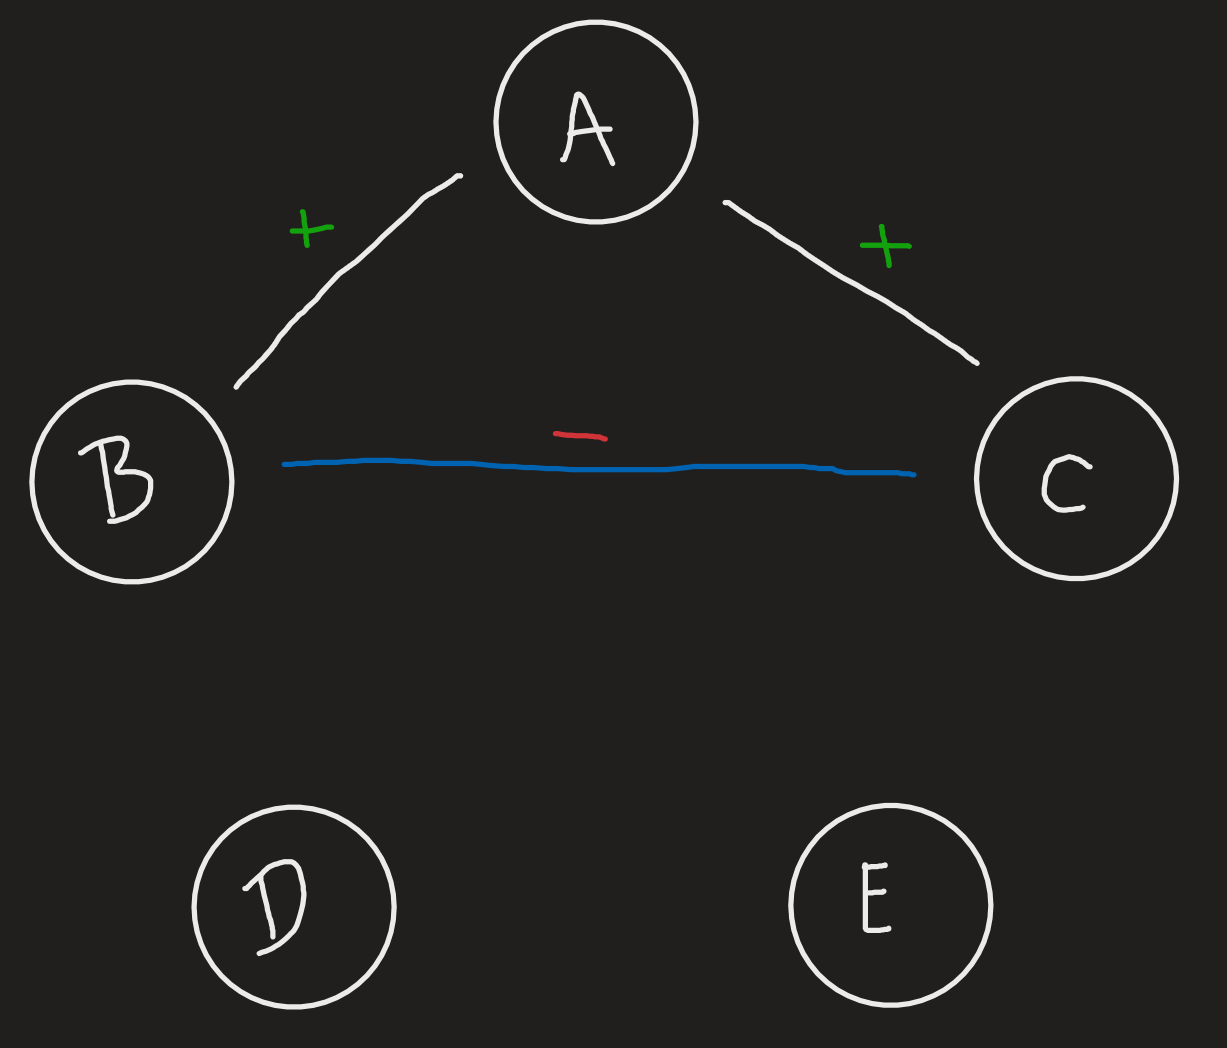
\includegraphics[scale=0.5]{Figure_3_2_4}\\
\end{center}
}

% Question 3
\item  When we think about structural balance, we can ask what happens when a new node tries to join a network in which there is existing friendship and hostility. In Figures 5.19-5.22, each pair of nodes is either friendly or hostile, as indicated by the + or - label on each edge.\\
% Uncomment to insert picture from Homeworkxx/Images
\begin{center}
	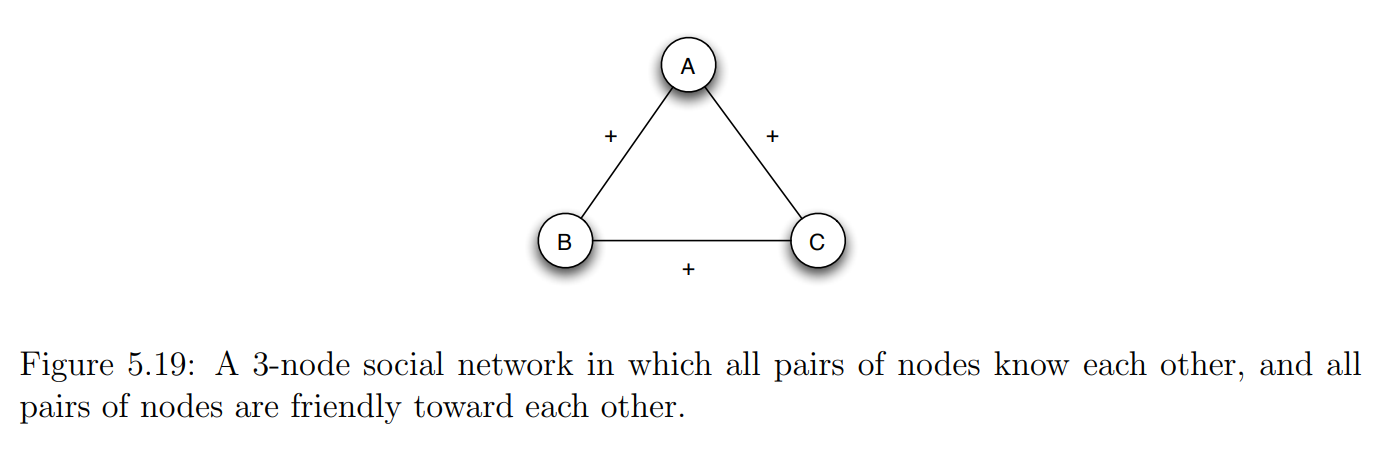
\includegraphics[scale=1]{Figure_5_19}\\
	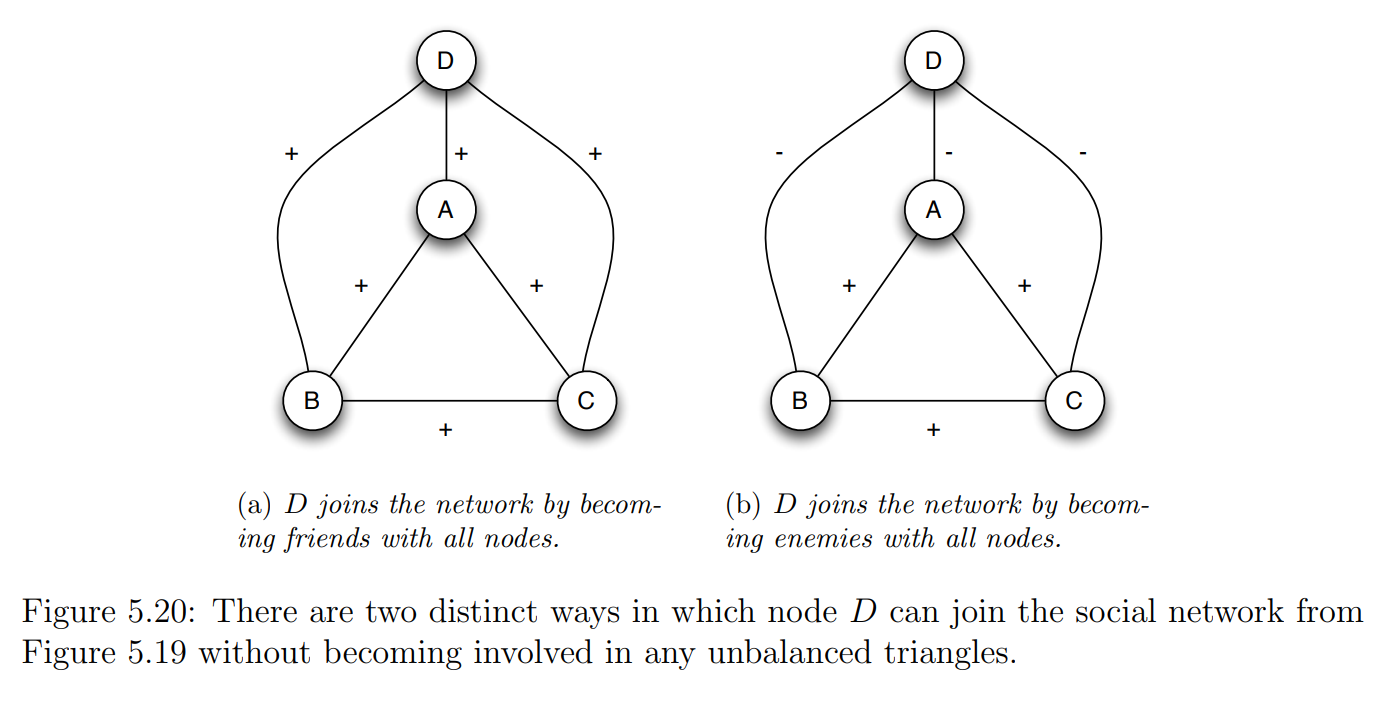
\includegraphics[scale=1]{Figure_5_19-20}\\
\end{center}
First, consider the 3-node social network in Figure 5.19, in which all pairs of nodes know each other, and all pairs of nodes are friendly toward each other. Now, a fourth node D wants to join this network, and establish either positive or negative relations with each existing node A, B, and C. It wants to do this in such a way that it doesn’t become involved in any unbalanced triangles. (I.e. so that after adding D and the labeled edges from D, there are no unbalanced triangles that contain D.) Is this possible?\\\\
In fact, in this example, there are two ways for D to accomplish this, as indicated in Figure 5.20. First, D can become friends with all existing nodes; in this way, all the triangles containing it have three positive edges, and so are balanced. Alternately, it can become enemies with all existing nodes; in this way, each triangle containing it has exactly one positive edge, and again these triangles would be balanced.\\\\
So for this network, it was possible for D to join without becoming involved in any unbalanced triangles. However, the same is not necessarily possible for other networks\\\\
We now consider this kind of question for some other networks.\\\\
\begin{center}
	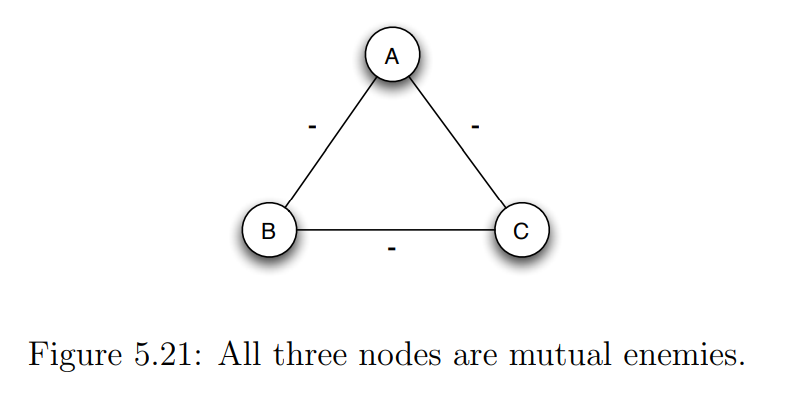
\includegraphics[scale=1]{Figure_5_21}\\
\end{center}
	\begin{enumerate}[(a)]
		% Question 3: Part 1
		\item Consider the 3-node social network in Figure 5.21, in which all pairs of nodes know each other, and each pair is either friendly or hostile as indicated by the + or - label on each edge. A fourth node D wants to join this network, and establish either positive or negative relations with each existing node A, B, and C. Can node D do this in such a way that it doesn’t become involved in any unbalanced triangles?\\
		\begin{enumerate}[*]
			\item  If there is a way for D to do this, say how many different such ways there are, and give an explanation. (That is, how many different possible labelings of the edges out of D have the property that all triangles containing D are balanced?)
			\item If there is no such way for D to do this, give an explanation why not. 
		\end{enumerate}
(In this and the subsequent questions, it possible to work out an answer by reasoning about the new node’s options without having to check all possibilities.\\
		% Question 3: Part 2
		\item Same question, but for a different network. Consider the 3-node social network in Figure 5.22, in which all pairs of nodes know each other, and each pair is either friendly or hostile as indicated by the + or - label on each edge. A fourth node D wants to join this network, and establish either positive or negative relations with each existing node A, B, and C. Can node D do this in such a way that it doesn’t become involved in any unbalanced triangles?
		\begin{enumerate}[*]
			\item  If there is a way for D to do this, say how many different such ways there are, and give an explanation. (That is, how many different possible labelings of the edges out of D have the property that all triangles containing D are balanced?)
			\begin{center}
				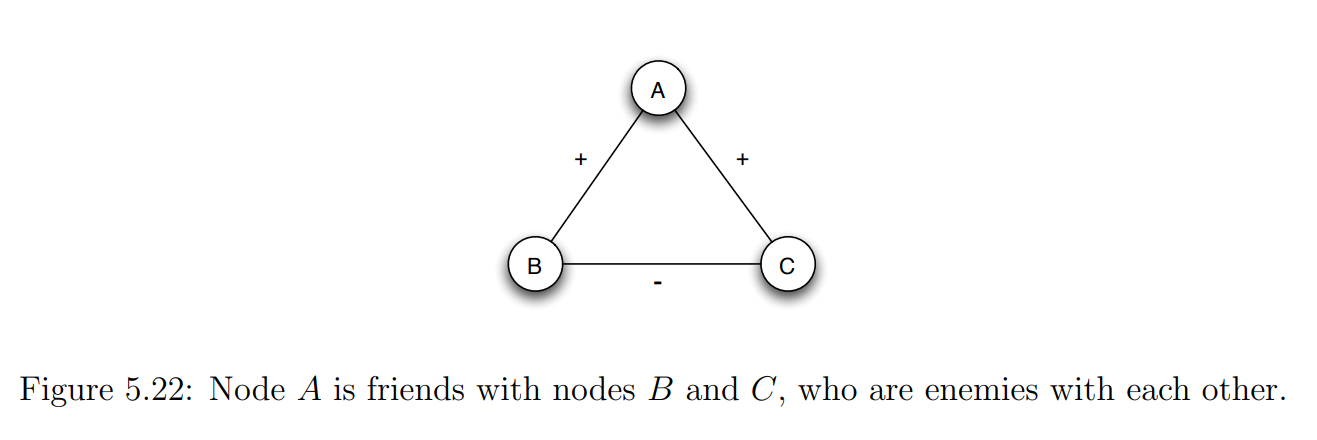
\includegraphics[scale=1]{Figure_5_22}\\
			\end{center}
			\item If there is no such way for D to do this, give an explanation why not.
		\end{enumerate}
		%Questions 3: Part 3
		\item Using what you’ve worked out in Questions 2 and 3, consider the following question. Take any labelled complete graph - on any number of nodes - that is not balanced; i.e. it contains at least one unbalanced triangle. (Recall that a labelled complete graph is a graph in which there is an edge between each pair of nodes, and each edge is labelled with either + or -.) A new node X wants to join this network, by attaching to each node using a positive or negative edge. When, if ever, is it possible for X to do this in such a way that it does not become involved in any unbalanced triangles? Give an explanation for your answer. (Hint: Think about any unbalanced triangle in the network, and how X must attach to the nodes in it.)
	\end{enumerate}
\end{enumerate}
\textcolor{gray}{
Answers:
\begin{enumerate}[(a)]
	\item PART A
	\item PART B
	\item PART C
\end{enumerate}}

\begin{enumerate} [\text{Canvas-}1.]
	% Canvas Question 1
	\item Consider the following graph:
	\begin{center}
		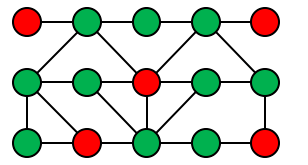
\includegraphics[scale=1]{canvas-1}\\
	\end{center}
 	Does this graph show evidence of homophily? Justify your answer from concepts we discussed in class.
\end{enumerate}
	\textcolor{gray}{
	Answers:
	\begin{enumerate} [\text{Canvas-}1.]
		\item something.
	\end {enumerate}}
\begin{enumerate} [\text{Canvas-}1.]
	\setcounter{enumi}{1} 
	% Canvas Question 2
	\item Consider the Schelling Segregation model we discussed in class. In class, we showed that if the contentedness threshold is 50\% (i.e., t=0.5, or I am content as long as at least half my Neighbors are my type), it's possible to create a long "row of houses" where everybody in society is content, and in which almost everybody has their maximum number of other-type friends (i.e., almost everybody has 50\% of their friends of a different type than themself).\\\\

Is it possible to extend this concept to other contentedness thresholds, and construct a society in which everybody is content, and almost everybody has a (1-t) fraction of their friends a different type than themself? For full credit, answer this for the specific values t=0.25 and t=0.75. For example, if t=0.25, can you construct a society in which everybody is content, and in which everybody (or almost everybody) has 75\% of their friends a different type than themself? Clearly explain any obstacles you encounter in completing this.\\
\end {enumerate}
	\textcolor{gray}{
	Answers:
	\begin{enumerate} [\text{Canvas-}1.]
	\setcounter{enumi}{1} 
		\item something.
	\end {enumerate}}

\end{document}
